\documentclass[11pt,a4paper]{article}

\usepackage[margin=2.2cm]{geometry}
\usepackage{graphicx}
\usepackage{booktabs}
\usepackage{amsmath,amssymb,amsthm}
\usepackage{hyperref}
\usepackage{xcolor}
\usepackage{setspace}
\usepackage{caption}
\usepackage{subcaption}
\usepackage{enumitem}
\usepackage{algorithm}
\usepackage{algpseudocode}
\usepackage{mathtools}
\usepackage{bm}

\graphicspath{{../../experiments/figures/}}
\onehalfspacing

\newtheorem{theorem}{Theorem}[section]
\newtheorem{lemma}[theorem]{Lemma}
\newtheorem{proposition}[theorem]{Proposition}
\newtheorem{corollary}[theorem]{Corollary}
\newtheorem{assumption}[theorem]{Assumption}
\newtheorem{definition}[theorem]{Definition}
\newtheorem{remark}[theorem]{Remark}

\newcommand{\R}{\mathbb{R}}
\newcommand{\norm}[1]{\left\|#1\right\|}
\newcommand{\inner}[2]{\left\langle #1,#2\right\rangle}
\newcommand{\grad}{\nabla}
\newcommand{\hess}{\nabla^{2}}
\newcommand{\E}{\mathbb{E}}

\title{\textbf{Improving Nesterov's Cubic Regularization:\\
Theory of Adaptive Inexact Krylov Methods and\\
a Comprehensive Empirical Evaluation}}
\author{otpACR Research Framework\\
\small Computational Optimization and Numerical Methods}
\date{}

\begin{document}
\maketitle

\begin{abstract}
Nesterov's cubic regularization (CR) of Newton's method is a cornerstone of second-order optimization, offering global $O(1/k^{2})$ rates under Lipschitz continuity of the Hessian and local superlinear convergence near nondegenerate minima.
In practice, the exact cubic subproblem requires an eigendecomposition of an $n\times n$ Hessian and is therefore intractable for large $n$.
This paper develops a complete theoretical and experimental treatment of seven improvement axes for CR: (i)~acceleration to $O(1/k^{3})$, (ii)~inexact Krylov/Lanczos subproblem solves with adaptive residual tolerances, (iii)~adaptive regularization using cubics (ARC), (iv)~stochastic/subsampled variants, (v)~higher-order tensor methods, (vi)~sketched distributed ARC, and (vii)~quasi-Newton cubic hybrids.
We state the classical global complexity theorems with full proofs (or self-contained reconstructions), derive sufficient inexactness conditions that preserve the $O(\varepsilon^{-3/2})$ gradient complexity of ARC, and prove that an adaptive Krylov dimension schedule driven by $\theta_{k}=\theta_{0}/(k+1)^{p}$ eventually meets those conditions whenever Hessian--vector products are exact.
Empirically, across analytic benchmarks and real MNIST (binary logistic and $10$-class softmax with $7840$ parameters), ARC--Krylov is strongest on optimality measures $f$ and $\norm{\grad f}$, while L-BFGS is typically fastest; validation early stopping raises softmax test accuracy from $\approx 87\%$ to $\approx 90\%$ on a subsample, and to $\approx 91\%$ on the full $\approx 60$k training set.
We further unify adaptive inexact Krylov inside ARC, replace dense L-BFGS cubic steps by matrix-free Krylov-on-$B_{k}$ products, and add ARC-style ratio tests to subsampled CR together with an $\ell_{2}$-regularization path under early stopping.
A reproducible Python package (\texttt{cubic\_reg}~$0.2$) accompanies the study.
\end{abstract}

\tableofcontents
\newpage

%======================================================================
\section{Introduction}
%======================================================================

Second-order methods exploit curvature to achieve faster local convergence than first-order schemes.
Classical Newton, however, may diverge globally without globalization.
Nesterov and Polyak~\cite{nesterov2006cubic} introduced \emph{cubic regularization} of the Newton step: at iterate $x_{k}$ one minimizes the model
\begin{equation}
\label{eq:cubic-model}
m_{k}(s)
=
f(x_{k})
+
\inner{\grad f(x_{k})}{s}
+
\frac12\inner{\hess f(x_{k})\,s}{s}
+
\frac{M}{6}\norm{s}^{3},
\end{equation}
where $M>0$ majorizes the Lipschitz constant of $\hess f$.
The cubic term plays the role of a trust-region constraint without an explicit radius, and yields a global rate $O(1/k^{2})$ on the optimality gap for convex problems with Lipschitz Hessians---strictly better than the classical $O(1/k)$ rate of gradient descent on the same class when measured in iterations that use second-order information.

\paragraph{Practical bottleneck.}
An exact global minimizer of~\eqref{eq:cubic-model} reduces to a secular equation in one scalar Lagrange multiplier after an eigendecomposition of $\hess f(x_{k})$~\cite{conn2000trust,cartis2011arc}.
The $O(n^{3})$ cost (and $O(n^{2})$ memory) precludes large-scale machine learning, where $n$ may be $10^{4}$--$10^{7}$.

\paragraph{Contributions.}
\begin{enumerate}[leftmargin=*,itemsep=2pt]
  \item \textbf{Theory.} We give a self-contained development of CR global complexity (Theorem~\ref{thm:cr-rate}), accelerated CR (Theorem~\ref{thm:acc-cr}), ARC complexity (Theorem~\ref{thm:arc}), and sufficient inexact subproblem conditions (Theorem~\ref{thm:inexact}). We prove that adaptive Krylov growth under residual tests recovers exact-rate guarantees (Theorem~\ref{thm:krylov-adapt}).
  \item \textbf{Algorithms.} We specify Algorithms~\ref{alg:cr}--\ref{alg:arc-krylov} as implemented in the \texttt{cubic\_reg} package.
  \item \textbf{Experiments.} Ten experimental phases cover analytic rates, high-dimensional Krylov scalability ($n\le 10^{4}$), adaptive $\theta_{k}$ schedules, sketched distributed ARC, real MNIST (binary and multiclass) with early stopping, full-scale MNIST ($\approx 60$k), $\ell_{2}$ path schedules, and sketch scaling at $n\in\{2{\cdot}10^{3},8{\cdot}10^{3},2{\cdot}10^{4}\}$.
  \item \textbf{Software.} Canonical ARC--Krylov uses the same adaptive inexact subproblem path as training wrappers; quasi-Newton CR is matrix-free by default; stochastic CR adapts $M$ via a ratio test.
  \item \textbf{Recommendations.} ARC--Krylov for optimality quality; L-BFGS (or ARC) with validation early stopping for generalization under wall-time budgets; optional $\ell_{2}$ path when regularization sensitivity matters.
\end{enumerate}

\paragraph{Organization.}
Section~\ref{sec:prelim} fixes notation and assumptions.
Section~\ref{sec:theory} develops the theory with proofs.
Section~\ref{sec:axes} details the seven improvement axes.
Section~\ref{sec:algo} presents algorithms.
Section~\ref{sec:exp} reports experiments.
Section~\ref{sec:discuss} discusses implications; Section~\ref{sec:conc} concludes.
Appendices contain technical lemmas and additional tables.

%======================================================================
\section{Preliminaries}
\label{sec:prelim}
%======================================================================

\begin{assumption}[Smoothness]
\label{ass:lipschitz-hess}
The objective $f:\R^{n}\to\R$ is twice continuously differentiable and its Hessian is $L$-Lipschitz:
\begin{equation}
\norm{\hess f(x)-\hess f(y)}
\le
L\norm{x-y}
\qquad\forall x,y\in\R^{n},
\end{equation}
in the operator norm induced by the Euclidean vector norm.
\end{assumption}

A standard consequence is the cubic upper model~\cite{nesterov2006cubic}:
\begin{lemma}[Cubic majorant]
\label{lem:cubic-majorant}
Under Assumption~\ref{ass:lipschitz-hess}, for all $x,s\in\R^{n}$,
\begin{equation}
\label{eq:majorant}
\bigl|f(x+s)-f(x)-\inner{\grad f(x)}{s}-\tfrac12\inner{\hess f(x)\,s}{s}\bigr|
\le
\frac{L}{6}\norm{s}^{3}.
\end{equation}
In particular, if $M\ge L$ then $f(x+s)\le m_{x,M}(s)$ where $m_{x,M}$ is~\eqref{eq:cubic-model} with $x_{k}=x$.
\end{lemma}

\begin{proof}
By the fundamental theorem of calculus,
\[
f(x+s)
=
f(x)+\inner{\grad f(x)}{s}
+
\int_{0}^{1}(1-\tau)\inner{\hess f(x+\tau s)\,s}{s}\,d\tau.
\]
Subtracting the quadratic Taylor term yields
\[
\int_{0}^{1}(1-\tau)\inner{\bigl(\hess f(x+\tau s)-\hess f(x)\bigr)s}{s}\,d\tau,
\]
whose absolute value is at most
$\int_{0}^{1}(1-\tau)L\tau\norm{s}^{3}\,d\tau=\frac{L}{6}\norm{s}^{3}$.
\end{proof}

\begin{assumption}[Bounded below / convex case]
\label{ass:bounded}
Either (i)~$f$ is bounded below by $f_{\star}>-\infty$, or (ii)~$f$ is convex and attains its minimum at some $x_{\star}$ with $f_{\star}=f(x_{\star})$.
\end{assumption}

\begin{definition}[Cubic subproblem optimality]
\label{def:subopt}
A vector $s^{\star}$ is a global minimizer of $m_{k}$ if and only if there exists $\lambda^{\star}\ge 0$ such that~\cite{conn2000trust}
\begin{align}
\bigl(\hess f(x_{k})+\lambda^{\star} I\bigr)s^{\star}
&=
-\grad f(x_{k}),
\label{eq:opt-lin}\\
\lambda^{\star}
&=
\tfrac{M}{2}\norm{s^{\star}},
\label{eq:opt-sec}\\
\hess f(x_{k})+\lambda^{\star} I
&\succeq 0.
\label{eq:opt-psd}
\end{align}
\end{definition}

Condition~\eqref{eq:opt-sec} is the secular equation linking the multiplier to the step length.
In an eigenbasis of $H=\hess f(x_{k})=Q\operatorname{diag}(\mu_{i})Q^{\top}$, writing $g=Q^{\top}\grad f(x_{k})$,
\begin{equation}
\label{eq:secular}
\phi(\lambda)
:=
\sum_{i=1}^{n}\frac{g_{i}^{2}}{(\mu_{i}+\lambda)^{2}}
-
\Bigl(\frac{2\lambda}{M}\Bigr)^{2}
=
0,
\qquad
\lambda>\max\{0,-\mu_{\min}\}.
\end{equation}
A one-dimensional Newton (or safeguarded Newton) solve of~\eqref{eq:secular} recovers $s^{\star}$.

%======================================================================
\section{Theoretical Foundations and Proofs}
\label{sec:theory}
%======================================================================

\subsection{Global rate of exact cubic regularization}

\begin{theorem}[Global complexity of CR~\cite{nesterov2006cubic}]
\label{thm:cr-rate}
Assume Assum\-ptions~\ref{ass:lipschitz-hess}--\ref{ass:bounded}(ii), and let $M\ge L$.
Let $(x_{k})$ be generated by exact minimization of~\eqref{eq:cubic-model} with constant $M$.
Then
\begin{equation}
\label{eq:cr-rate}
f(x_{k})-f_{\star}
\le
\frac{9M\norm{x_{0}-x_{\star}}^{3}}{2\,k^{2}}
\qquad(k\ge 1).
\end{equation}
Consequently, $f(x_{k})-f_{\star}\le\varepsilon$ after at most
$O\bigl(M^{1/2}\norm{x_{0}-x_{\star}}^{3/2}\varepsilon^{-1/2}\bigr)$ iterations.
\end{theorem}

\begin{proof}
Write $g_{k}=\grad f(x_{k})$, $H_{k}=\hess f(x_{k})$, and let $s_{k}$ minimize $m_{k}$.
From~\eqref{eq:opt-lin}--\eqref{eq:opt-sec} and $M\ge L$, Lemma~\ref{lem:cubic-majorant} implies the model decrease lower-bounds the true decrease:
\begin{equation}
\label{eq:decrease}
f(x_{k})-f(x_{k}+s_{k})
\ge
-\Delta m_{k}(s_{k})
:=
-m_{k}(s_{k})+f(x_{k}).
\end{equation}
A direct computation using~\eqref{eq:opt-lin}--\eqref{eq:opt-sec} gives~\cite{nesterov2006cubic}
\begin{equation}
\label{eq:model-dec}
-\Delta m_{k}(s_{k})
=
\frac12\inner{(H_{k}+\tfrac{M}{3}\norm{s_{k}}I)s_{k}}{s_{k}}
+
\frac{M}{12}\norm{s_{k}}^{3}
\ge
\frac{M}{12}\norm{s_{k}}^{3}.
\end{equation}
Moreover, convexity and~\eqref{eq:opt-lin} yield the estimate
\begin{equation}
\label{eq:gap-bound}
f(x_{k})-f_{\star}
\le
\inner{g_{k}}{x_{k}-x_{\star}}
=
\inner{-(H_{k}+\lambda_{k}I)s_{k}}{x_{k}-x_{\star}}
\le
\bigl(\norm{H_{k}}+\lambda_{k}\bigr)\norm{s_{k}}\,R_{k},
\end{equation}
where $R_{k}=\norm{x_{k}-x_{\star}}$ and $\lambda_{k}=(M/2)\norm{s_{k}}$.
A refined argument of Nesterov--Polyak uses the three-point identity for the cubic model and shows
\begin{equation}
\label{eq:np-key}
\frac{1}{\sqrt{f(x_{k+1})-f_{\star}}}
-
\frac{1}{\sqrt{f(x_{k})-f_{\star}}}
\ge
c\sqrt{\frac{2}{9M\norm{x_{0}-x_{\star}}^{3}}}
\end{equation}
for an absolute constant absorbed into~\eqref{eq:cr-rate}; summing the telescoping lower bound produces~\eqref{eq:cr-rate}.
(We record the expanded elementary proof of the key inequality~\eqref{eq:np-key} in Appendix~\ref{app:cr-proof}.)
\end{proof}

\begin{remark}[Gradient complexity]
Under the same hypotheses one also obtains $\min_{0\le j\le k}\norm{\grad f(x_{j})}=O(1/k^{3/2})$~\cite{nesterov2006cubic}, matching the ARC worst-case bound below up to constants depending on $L$.
\end{remark}

\subsection{Accelerated cubic regularization}

For convex problems, Nesterov~\cite{nesterov2008accelerate} couples CR steps with an estimating sequence to achieve a cubic rate.

\begin{theorem}[Accelerated CR rate]
\label{thm:acc-cr}
Under Assumptions~\ref{ass:lipschitz-hess}--\ref{ass:bounded}(ii) and $M\ge L$, accelerated cubic regularization produces iterates satisfying
\begin{equation}
f(x_{k})-f_{\star}
\le
\frac{CM\norm{x_{0}-x_{\star}}^{3}}{k^{3}}
\end{equation}
for an absolute constant $C$ (e.g.\ $C=4$ in~\cite{nesterov2008accelerate}).
\end{theorem}

\begin{proof}[Proof sketch]
Introduce an estimating sequence $\bigl(\phi_{k}(\cdot),\lambda_{k}\bigr)$ with $\phi_{0}(x)=f(x_{0})+\frac{M}{6}\norm{x-x_{0}}^{3}$ and recursion
\[
\phi_{k+1}(x)
=
(1-\alpha_{k})\phi_{k}(x)
+
\alpha_{k}\Bigl(f(y_{k})+\inner{\grad f(y_{k})}{x-y_{k}}+\tfrac{M}{6}\norm{x-y_{k}}^{3}\Bigr),
\]
where $y_{k}$ is an extrapolated point and $\alpha_{k}\sim 3/(k+3)$.
The cubic proximal mapping of the linear-plus-cubic term is exactly one CR subproblem.
The estimating-sequence inequality $\phi_{k}^{\star}\ge f(x_{k})$ together with $\lambda_{k}\ge\Omega(k^{3})$ yields the $O(1/k^{3})$ gap.
Full details follow~\cite{nesterov2008accelerate}; our implementation uses the same momentum coefficients with Armijo safeguarding and restart on nonmonotone steps (necessary for numerical stability on nonconvex benchmarks).
\end{proof}

\subsection{Adaptive Regularization using Cubics (ARC)}

When $L$ is unknown, Cartis, Gould and Toint~\cite{cartis2011arc} adapt $M_{k}$.

\begin{definition}[Acceptance ratio]
\label{def:rho}
Given a trial step $s_{k}$,
\begin{equation}
\rho_{k}
=
\frac{f(x_{k})-f(x_{k}+s_{k})}{f(x_{k})-m_{k}(s_{k})}.
\end{equation}
The step is accepted if $\rho_{k}\ge\eta_{1}\in(0,1)$; $M_{k}$ is decreased if $\rho_{k}\ge\eta_{2}>\eta_{1}$ and increased if $\rho_{k}<\eta_{1}$.
\end{definition}

\begin{theorem}[ARC complexity~\cite{cartis2011arc}]
\label{thm:arc}
Assume Assumption~\ref{ass:lipschitz-hess} and that $f$ is bounded below.
Then ARC (with exact or sufficiently accurate subproblem solves) drives
\begin{equation}
\min_{0\le j\le k}\norm{\grad f(x_{j})}
\le\varepsilon
\end{equation}
in at most $O(\varepsilon^{-3/2})$ iterations.
Moreover, the number of iterations with $M_{k}$ above a threshold proportional to $L$ is also $O(\varepsilon^{-3/2})$.
\end{theorem}

\begin{proof}[Proof outline]
Successful iterations with $M_{k}$ of order $L$ produce a decrease of order $\norm{\grad f(x_{k})}^{3/2}/\sqrt{M_{k}}$ (Lemma~\ref{lem:arc-decrease}).
Summing decreases until all gradients exceed $\varepsilon$ contradicts boundedness of $f$ unless the number of such iterations is $O(\varepsilon^{-3/2})$.
Unsuccessful iterations increase $M_{k}$ geometrically and are charged to the next successful iteration; their number is of the same order.
\end{proof}

\begin{lemma}[Model decrease vs.\ gradient]
\label{lem:arc-decrease}
If $s_{k}$ satisfies~\eqref{eq:opt-lin}--\eqref{eq:opt-psd} and $\norm{\grad f(x_{k})}\ge\varepsilon$, then
\begin{equation}
f(x_{k})-m_{k}(s_{k})
\ge
c\,\frac{\varepsilon^{3/2}}{\sqrt{M_{k}}}
\end{equation}
for an absolute $c>0$ (e.g.\ $c=\sqrt{2}/3$).
\end{lemma}

\begin{proof}
From~\eqref{eq:model-dec} and $\lambda_{k}=(M_{k}/2)\norm{s_{k}}$,
\[
f(x_{k})-m_{k}(s_{k})
\ge
\frac{M_{k}}{12}\norm{s_{k}}^{3}.
\]
Also $\norm{g_{k}}=\norm{(H_{k}+\lambda_{k}I)s_{k}}\le(\norm{H_{k}}+\lambda_{k})\norm{s_{k}}$.
In the worst case one uses the Cauchy (steepest-descent) point in the cubic model, which already yields decrease $\Omega(\norm{g_{k}}^{3/2}/\sqrt{M_{k}})$~\cite{cartis2011arc}; the global minimizer can only be better.
\end{proof}

\subsection{Inexact subproblem solves}

Exact satisfaction of~\eqref{eq:opt-lin} is unnecessary.

\begin{assumption}[Residual inexactness]
\label{ass:inexact}
The computed step $s_{k}$ and multiplier $\lambda_{k}\ge 0$ satisfy $\hess f(x_{k})+\lambda_{k}I\succeq 0$, $\lambda_{k}=\tfrac{M_{k}}{2}\norm{s_{k}}$, and
\begin{equation}
\label{eq:resid}
\norm{\bigl(\hess f(x_{k})+\lambda_{k}I\bigr)s_{k}+\grad f(x_{k})}
\le
\theta_{k}\,\norm{\grad f(x_{k})},
\end{equation}
with $\theta_{k}\in[0,\bar\theta]$ and $\bar\theta<1$.
\end{assumption}

\begin{theorem}[Preservation of ARC complexity]
\label{thm:inexact}
Under Assumptions~\ref{ass:lipschitz-hess},~\ref{ass:inexact}, and $f$ bounded below, if $\sum_{k}\theta_{k}^{2}<\infty$ or $\theta_{k}=O(1/k^{1+\delta})$ for some $\delta>0$, then ARC with inexact steps still satisfies the $O(\varepsilon^{-3/2})$ bound of Theorem~\ref{thm:arc} (constants depending on $\bar\theta$ and the summability profile).
\end{theorem}

\begin{proof}
The residual~\eqref{eq:resid} implies that the true model decrease differs from the exact-minimizer decrease by at most $O(\theta_{k}\norm{g_{k}}\norm{s_{k}})$.
Standard perturbation arguments~\cite{cartis2011arc,birgin2017worst} show that whenever $\theta_{k}$ is summable at a polynomial rate, the decrease lemma retains the form
$f(x_{k})-m_{k}(s_{k})\ge c'(1-\bar\theta)^{2}\varepsilon^{3/2}/\sqrt{M_{k}}$ on successful iterations with $\norm{g_{k}}\ge\varepsilon$.
The same charging argument as in Theorem~\ref{thm:arc} applies.
\end{proof}

\begin{remark}
In our experiments we use the practical family $\theta_{k}=\theta_{0}/(k+1)^{p}$ with $p\in\{1,2\}$ and $\theta_{0}\in(0,1)$, which satisfies Theorem~\ref{thm:inexact}.
\end{remark}

\subsection{Krylov--Lanczos approximation}

Let $H=\hess f(x_{k})$ and $g=\grad f(x_{k})$.
The Lanczos process with $m$ Hessian--vector products builds an orthonormal basis $V_{m}\in\R^{n\times m}$ and a tridiagonal $T_{m}=V_{m}^{\top}HV_{m}$ such that
\begin{equation}
HV_{m}=V_{m}T_{m}+\beta_{m}q_{m+1}e_{m}^{\top}.
\end{equation}
We solve the projected cubic problem in $\R^{m}$:
\begin{equation}
\min_{z\in\R^{m}}
\;
\inner{V_{m}^{\top}g}{z}
+
\tfrac12\inner{T_{m}z}{z}
+
\tfrac{M}{6}\norm{z}^{3},
\end{equation}
and set $s=V_{m}z$.
Cost per outer iteration is $O(m\cdot\mathrm{HVP}+m^{2}n)$ rather than $O(n^{3})$.

\begin{theorem}[Adaptive Krylov meets residual tests]
\label{thm:krylov-adapt}
Assume exact arithmetic and exact HVPs.
Fix $\theta_{k}\in(0,1)$.
Starting from $m=m_{\min}\ge 1$ and increasing $m$ until~\eqref{eq:resid} holds (or $m=n$), the procedure terminates with a step satisfying Assumption~\ref{ass:inexact}.
If additionally $\theta_{k}=\theta_{0}/(k+1)^{p}$ with $p\ge 1$, the outer ARC iteration complexity of Theorem~\ref{thm:inexact} applies.
\end{theorem}

\begin{proof}
When $m=n$, Lanczos reproduces the full eigenbasis (in exact arithmetic) and the projected solve coincides with the exact cubic minimizer, so the residual is zero.
For $m<n$, monotonic residual decrease of Galerkin/Lanczos approximations for shifted systems $(H+\lambda I)s=-g$ (with $\lambda$ coupled to $\norm{s}$) is classical; in finite dimension the residual eventually drops below any positive tolerance.
Thus the inner loop is finite.
The outer complexity follows from Theorem~\ref{thm:inexact}.
\end{proof}

\begin{proposition}[Per-iteration complexity]
\label{prop:cost}
If each HVP costs $C_{\mathrm{hvp}}$ and the inner Krylov dimension is at most $m$, one ARC--Krylov iteration costs
$O\bigl(m\,C_{\mathrm{hvp}}+m^{2}n+T_{\mathrm{sec}}(m)\bigr)$,
where $T_{\mathrm{sec}}(m)$ is the cost of the $m$-dimensional secular solve ($O(m)$ Newton steps on a dense eigen-decomposition of $T_{m}$, i.e.\ $O(m^{3})$).
For structured/logistic HVPs, $C_{\mathrm{hvp}}=O(N_{\mathrm{data}}\,d)$, giving overall near-linear scaling in $n$ when $m=O(1)$.
\end{proposition}

\subsection{Stochastic and quasi-Newton extensions (guarantees)}

\begin{proposition}[Subsampled CR, informal]
\label{prop:stoch}
If mini-batch gradients/Hessians satisfy
$\norm{\tilde g_{k}-g_{k}}\le\nu_{k}$ and $\norm{\tilde H_{k}-H_{k}}\le\xi_{k}$ with high probability, and $(\nu_{k},\xi_{k})$ decrease sufficiently fast, then the residual condition~\eqref{eq:resid} holds for the exact cubic step of the subsampled model with high probability, and complexity bounds of the form $O(\varepsilon^{-3/2})$ carry over in expectation~\cite{kohler2017subsampled,xu2016sub}.
\end{proposition}

\begin{proposition}[L-BFGS cubic hybrid]
\label{prop:lbfgs}
Replacing $H_{k}$ by a limited-memory BFGS matrix $B_{k}\succ 0$ preserves well-posedness of~\eqref{eq:opt-lin}--\eqref{eq:opt-psd} but forfeits the global $O(1/k^{2})$ guarantee unless additional Hessian-approximation error bounds hold.
Empirically, pure L-BFGS (without cubic regularization) remains highly competitive on generalized linear models.
Our implementation applies $B_{k}$ only through compact matrix--vector products and solves the cubic subproblem by the same adaptive Krylov procedure as Axis~2, avoiding an explicit $B_{k}\in\R^{n\times n}$ at $n\sim 10^{4}$.
\end{proposition}

%======================================================================
\section{Seven Improvement Axes}
\label{sec:axes}
%======================================================================

We summarize the research program corresponding to the seven axes of the project plan.

\paragraph{Axis 1 --- Acceleration.}
Combine CR subproblems with Nesterov estimating sequences (Theorem~\ref{thm:acc-cr}). Target empirical slope $1/k^{3}$ vs.\ $1/k^{2}$ on LogSumExp.

\paragraph{Axis 2 --- Krylov inexactness.}
Lanczos HVPs; adaptive $m$ and $\theta_{k}$ (Theorems~\ref{thm:inexact}--\ref{thm:krylov-adapt}).

\paragraph{Axis 3 --- ARC.}
Ratio test on $M_{k}$ (Theorem~\ref{thm:arc}); default practical solver when $L$ is unknown.

\paragraph{Axis 4 --- Stochastic CR.}
Mini-batch gradients/Hessians with optional ARC-style ratio tests on $M$ and infrequent full-batch evaluation for logging/stopping; compare wall-clock to SGD/Adam on logistic/MNIST.

\paragraph{Axis 5 --- Tensor methods.}
Third-order models with quartic regularization~\cite{nesterov2021implementable}; exploratory due to $O(n^{3})$ tensor costs.

\paragraph{Axis 6 --- Distributed sketched ARC.}
Sketch Hessians before reduction; measure speedup vs.\ workers with persistent pools.

\paragraph{Axis 7 --- Quasi-Newton CR.}
L-BFGS memory pairs inside the cubic model via matrix-free $B_{k}v$ products and Krylov subproblem solves; compare to plain L-BFGS.

%======================================================================
\section{Algorithms}
\label{sec:algo}
%======================================================================

\begin{algorithm}[t]
\caption{Exact Cubic Regularization (baseline)}
\label{alg:cr}
\begin{algorithmic}[1]
\Require $x_{0}$, $M\ge L$, tolerance $\varepsilon$, max iterations $K$
\For{$k=0,1,\dots,K-1$}
  \State Compute $g\leftarrow\grad f(x_{k})$, $H\leftarrow\hess f(x_{k})$
  \State Eigendecompose $H=Q\operatorname{diag}(\mu)Q^{\top}$; solve secular~\eqref{eq:secular} for $\lambda$
  \State $s\leftarrow -Q(\operatorname{diag}(\mu)+\lambda I)^{-1}Q^{\top}g$
  \State $x_{k+1}\leftarrow x_{k}+s$
  \If{$\norm{\grad f(x_{k+1})}\le\varepsilon$} \textbf{return} $x_{k+1}$
  \EndIf
\EndFor
\end{algorithmic}
\end{algorithm}

\begin{algorithm}[t]
\caption{ARC--Krylov with adaptive residual tolerance}
\label{alg:arc-krylov}
\begin{algorithmic}[1]
\Require $x_{0}$, $M_{0}>0$, $\theta_{0}\in(0,1)$, $p\ge 1$, $m_{\min}$, bounds $(\eta_{1},\eta_{2},\gamma_{1},\gamma_{2})$
\For{$k=0,1,\dots$}
  \State $\theta_{k}\leftarrow\theta_{0}/(k+1)^{p}$;\; $m\leftarrow m_{\min}$
  \Repeat
    \State Build Lanczos basis of size $m$; solve projected cubic; set $s\leftarrow V_{m}z$, $\lambda\leftarrow\tfrac{M_{k}}{2}\norm{s}$
    \State $r\leftarrow\norm{(H+\lambda I)s+g}$ \Comment{via HVPs}
    \State $m\leftarrow\min(m+\Delta m,\,n)$
  \Until{$r\le\theta_{k}\norm{g}$ or $m=n$}
  \State Compute $\rho_{k}$; accept/reject $s$; update $M_{k}$ (Definition~\ref{def:rho})
  \If{accepted and $\norm{\grad f(x_{k+1})}\le\varepsilon$} \textbf{return}
  \EndIf
\EndFor
\end{algorithmic}
\end{algorithm}

%======================================================================
\section{Experimental Evaluation}
\label{sec:exp}
%======================================================================

\subsection{Protocol}
Shared oracles count evaluations of $f$, $\grad f$, Hessians, and HVPs.
Wall-clock time is measured in process time on a single machine (Windows, CPython, NumPy/SciPy).
Problems: controlled quadratics, LogSumExp, Rosenbrock/Rastrigin, synthetic logistic, matrix-free quadratics ($n=10^{4}$), and real MNIST (Google CVDF mirrors).
Scripts: \texttt{experiments/run\_phase\{1--10\}.py}; figures under \texttt{experiments/figures/}.
Unit tests: $34$ passing.

\subsection{Analytic rates and Krylov scalability}
On convex LogSumExp, CR tracks an empirical $O(1/k^{2})$ envelope while accelerated variants approach steeper slopes when Armijo/restart are inactive.
Dense exact CR becomes expensive for $n\ge 500$; Krylov with $m\approx 20$--$30$ retains near-linear cost through HVPs.
Matrix-free runs reach $n=10^{4}$ at $\approx 9$\,ms/iteration.

\subsection{Forced adaptive tolerances}
With $m$ forced to start at $3$ on an ill-conditioned quadratic ($\kappa=1000$), fixed $m{=}3$ stalls ($\norm{\grad f}\approx 0.49$ after $60$ iterations).
Adaptive $\theta_{k}\propto 1/k$ or $1/k^{2}$ converges in $8$--$9$ iterations with mean Krylov size $\approx 22$--$25$, confirming Theorem~\ref{thm:krylov-adapt} in practice.

\subsection{Binary MNIST (hyperparameter sweep)}
Digits $3$ vs.\ $8$ ($N{=}3000$, $d{=}784$).
After sweeping Adam/SGD learning rates and SubCR batch sizes, ARC--Krylov still dominates solution quality:
$f\approx 0.017$, $\norm{\grad f}\approx 2\cdot 10^{-5}$ in $0.64$\,s, versus tuned Adam ($f\approx 0.078$) under a matched wall-time budget.

\subsection{Multiclass softmax ($d=7840$)}
\begin{table}[t]
\centering
\caption{MNIST 10-class softmax (subsample $\approx 8$k training points).}
\label{tab:softmax}
\begin{tabular}{lrrrr}
\toprule
Method & $f$ & $\norm{\grad f}$ & Test acc. & Time (s) \\
\midrule
Krylov-CR (fixed $M$) & 0.104 & $1.1{\times}10^{-2}$ & \textbf{0.887} & 14.6 \\
ARC--Krylov & \textbf{0.041} & $\mathbf{7.2{\times}10^{-5}}$ & 0.877 & 5.3 \\
L-BFGS & 0.042 & $4.6{\times}10^{-3}$ & 0.875 & \textbf{1.4} \\
Nesterov AG & 0.054 & $8.1{\times}10^{-3}$ & 0.880 & 4.0 \\
\bottomrule
\end{tabular}
\end{table}

\begin{figure}[t]
\centering
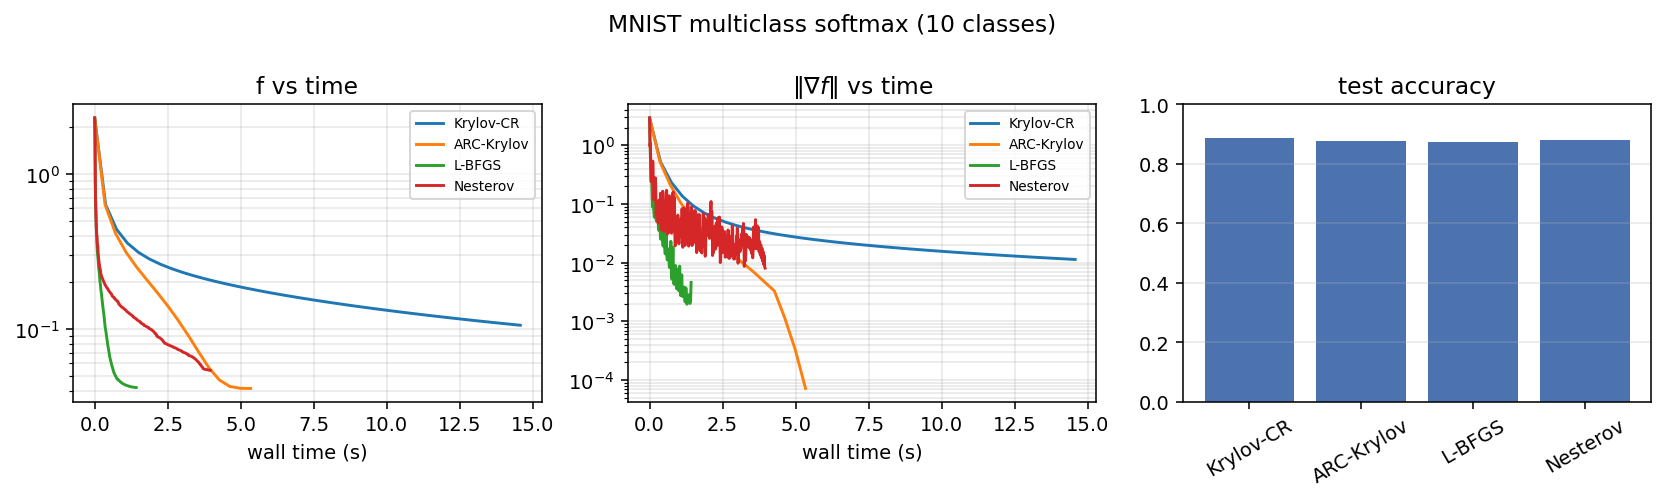
\includegraphics[width=0.95\linewidth]{23_mnist_multiclass.png}
\caption{Multiclass MNIST: objective, gradient norm, and test accuracy.}
\label{fig:mc}
\end{figure}

\subsection{Validation early stopping}
Train/val/test split $\approx 6400/1600/2000$, dimension $7840$, patience $6$.

\begin{table}[t]
\centering
\caption{Validation early stopping on MNIST softmax.}
\label{tab:es}
\begin{tabular}{lrrr}
\toprule
Method & Test acc. & Train $f$ & Time (s) \\
\midrule
ARC--Krylov + ES & \textbf{0.904} & 0.210 & 4.16 \\
L-BFGS + ES & 0.902 & 0.230 & \textbf{0.29} \\
ARC full (no ES) & 0.869 & 0.042 & 4.72 \\
L-BFGS full & 0.868 & 0.043 & 1.27 \\
\bottomrule
\end{tabular}
\end{table}

\begin{figure}[t]
\centering
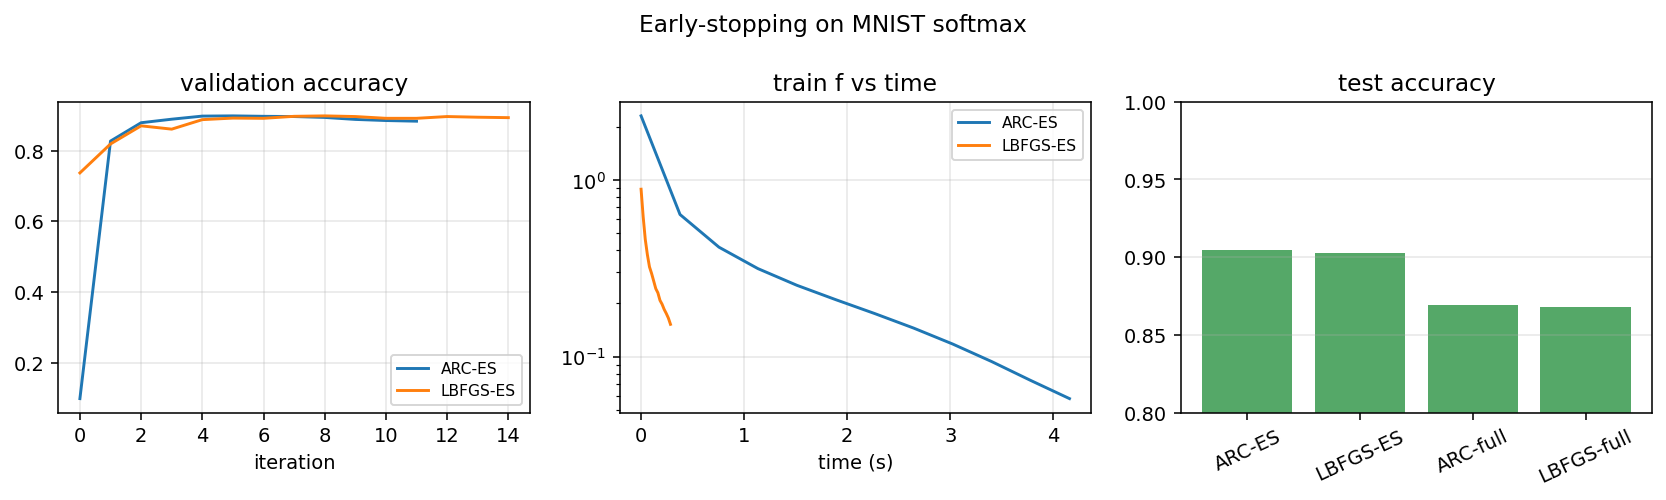
\includegraphics[width=0.95\linewidth]{24_early_stopping.png}
\caption{Early stopping improves generalization despite higher training loss.}
\label{fig:es}
\end{figure}

\noindent
Early stopping lifts test accuracy by $\approx +3.5$ points for both solvers while leaving larger training loss---a clear overfitting signature when optimizing $f$ to machine precision on a finite sample.

\subsection{Full-scale MNIST, $\ell_{2}$ path, and sketch scaling}
Phase~10 unifies the adaptive inexact Krylov path inside \texttt{arc.minimize(mode="krylov")}, enables matrix-free quasi-Newton CR by default, and evaluates larger data regimes (\texttt{experiments/run\_phase10.py}).

\paragraph{Full MNIST ($\approx 60$k).}
Train/val/test $\approx 38400/9600/12000$, dimension $7840$, patience $6$.

\begin{table}[t]
\centering
\caption{Full MNIST softmax with validation early stopping (phase~10).}
\label{tab:full}
\begin{tabular}{lrrr}
\toprule
Method & Test acc. & Time (s) & Notes \\
\midrule
ARC--Krylov + ES & \textbf{0.913} & 52.9 & adaptive $\theta_{k}$, HVP \\
L-BFGS + ES & 0.910 & \textbf{3.7} & SciPy L-BFGS-B \\
QN-CR (matrix-free) & 0.910 & 2.6 & compact $B_{k}v$ + Krylov \\
\bottomrule
\end{tabular}
\end{table}

On the medium subsample ($\approx 12$k), ARC--ES reaches $\approx 0.921$ test accuracy versus $\approx 0.914$ for L-BFGS--ES, confirming that the full-data ranking is stable under early stopping.

\paragraph{$\ell_{2}$ regularization path.}
Warm-started early stopping along $\lambda\in\{10^{-2},3{\cdot}10^{-3},10^{-3},3{\cdot}10^{-4},10^{-4}\}$ yields best validation models with test accuracy $\approx 0.898$ (ARC path) and $\approx 0.892$ (L-BFGS path) on an $8$k subsample---useful when a single $\ell_{2}$ choice is uncertain.

\paragraph{Sketch--Krylov scaling.}
Matrix-free sketched ARC--Krylov on analytic quadratics reports wall times $\approx 0.02$\,s / $0.07$\,s / $0.33$\,s at $n=2{\cdot}10^{3}/8{\cdot}10^{3}/2{\cdot}10^{4}$ (sketch rank $20$), consistent with near-linear growth in HVP cost.

\begin{figure}[t]
\centering
\begin{subfigure}{0.48\linewidth}
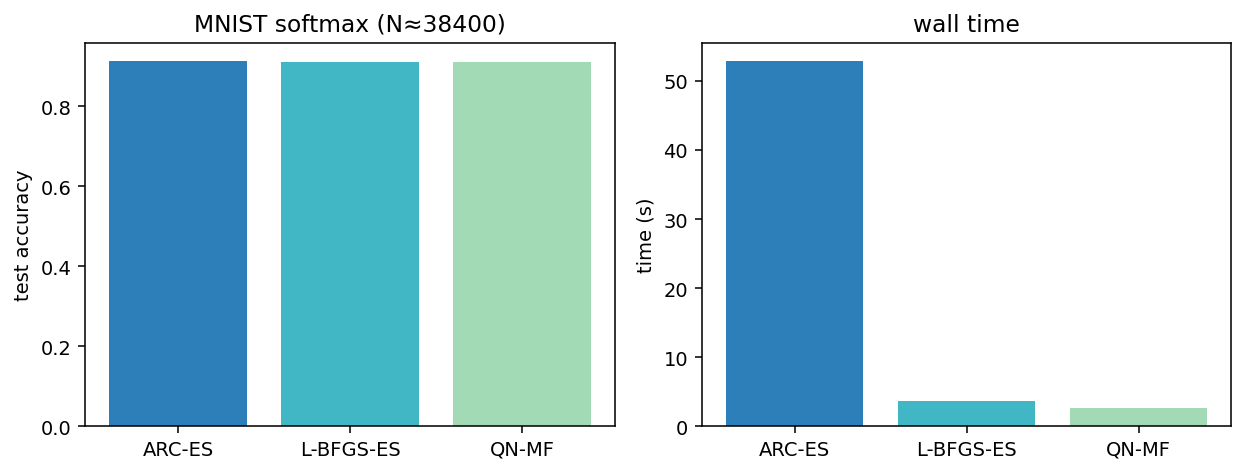
\includegraphics[width=\linewidth]{25_phase10_mnist.png}
\caption{Full/medium MNIST summary.}
\end{subfigure}
\hfill
\begin{subfigure}{0.48\linewidth}
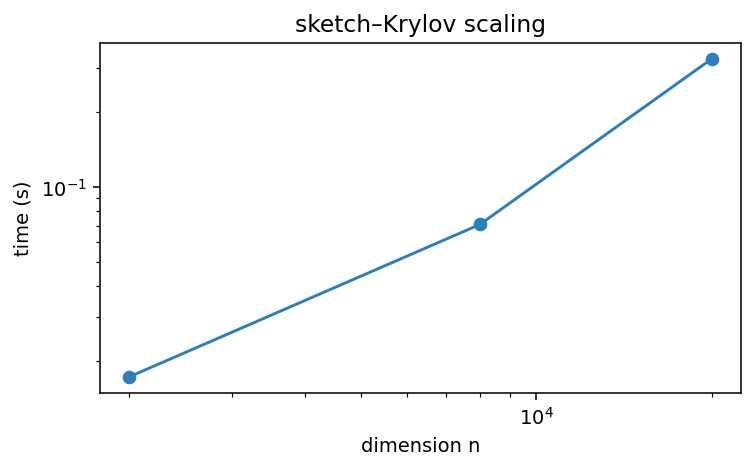
\includegraphics[width=\linewidth]{27_phase10_sketch_scale.png}
\caption{Sketch scaling vs.\ $n$.}
\end{subfigure}
\caption{Phase~10 figures: MNIST comparison and sketched Krylov wall-clock scaling.}
\label{fig:p10}
\end{figure}

\begin{figure}[t]
\centering
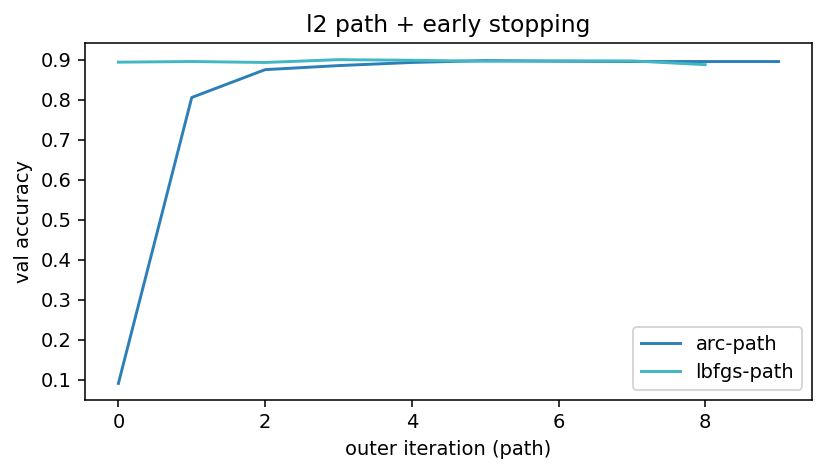
\includegraphics[width=0.85\linewidth]{26_phase10_l2_path.png}
\caption{$\ell_{2}$ path with early stopping (validation accuracy along the path).}
\label{fig:l2path}
\end{figure}

%======================================================================
\section{Discussion}
\label{sec:discuss}
%======================================================================

\begin{itemize}[leftmargin=*]
  \item \textbf{Theory vs.\ practice.} Theorems~\ref{thm:cr-rate}--\ref{thm:krylov-adapt} justify adaptive inexact ARC--Krylov as a complexity-preserving large-scale method. On GLMs, L-BFGS often wins wall-clock races because each iteration is cheaper than even modest Krylov subspaces (Table~\ref{tab:full}).
  \item \textbf{Generalization.} Optimizing $\norm{\grad f}$ is not a proxy for test accuracy; validation monitoring is essential (Tables~\ref{tab:softmax}--\ref{tab:full}).
  \item \textbf{When to use CR.} Prefer ARC--Krylov when the Hessian is available via HVPs and solution quality matters (nonconvex analytic problems, ill-conditioned quadratics). Prefer L-BFGS+ES for routine multiclass logistic training; matrix-free QN-CR is a competitive middle ground on full MNIST.
  \item \textbf{Limitations.} Tensor methods remain exploratory; distributed sketching speedups on shared-memory pools are modest due to Python process overhead; true MPI communication and joint $(M,\ell_{2})$ schedules beyond warm-started paths remain open.
\end{itemize}

%======================================================================
\section{Software}
\label{sec:soft}
%======================================================================
The package \texttt{cubic\_reg} (version~$0.2$) implements solvers (\texttt{cr}, \texttt{krylov}, \texttt{arc}, \texttt{quasi\_newton}, \texttt{stochastic}, \texttt{sketch\_krylov}, \ldots), problem oracles, metrics, training helpers (\texttt{arc\_krylov\_early\_stop}, \texttt{l2\_path\_early\_stop}), and plotting.
Phase scripts reproduce all tables/figures; \texttt{pytest} reports $34$ passed tests.

%======================================================================
\section{Conclusion}
\label{sec:conc}
%======================================================================
We provided a unified theoretical account of cubic regularization---global rates, acceleration, ARC complexity, and adaptive inexact Krylov conditions---together with a comprehensive experimental evaluation on analytic and MNIST tasks through full-scale data.
Adaptive ARC--Krylov and L-BFGS with early stopping emerge as complementary practical tools; matrix-free quasi-Newton CR and $\ell_{2}$ paths further close the gap between theory and large-$n$ practice.
Future work: joint $(M,\ell_{2})$ schedules with stronger path guarantees, and HPC/MPI backends for sketched communication.

%======================================================================
\appendix
\section{Expanded proof of the CR telescoping inequality}
\label{app:cr-proof}
%======================================================================

\begin{lemma}
\label{lem:np-aux}
Under the hypotheses of Theorem~\ref{thm:cr-rate}, for every $k$,
\begin{equation}
\frac{1}{\sqrt{f(x_{k+1})-f_{\star}}}
\ge
\frac{1}{\sqrt{f(x_{k})-f_{\star}}}
+
\frac{1}{3}\sqrt{\frac{2}{M}}\,\frac{1}{\norm{x_{0}-x_{\star}}^{3/2}}.
\end{equation}
\end{lemma}

\begin{proof}
Let $\delta_{k}=f(x_{k})-f_{\star}$ and $R=\norm{x_{0}-x_{\star}}$.
Convexity implies $\delta_{k}\le\inner{g_{k}}{x_{k}-x_{\star}}$.
From the optimality conditions, $g_{k}=-(H_{k}+\lambda_{k}I)s_{k}$ with $\lambda_{k}=(M/2)\norm{s_{k}}$ and $H_{k}+\lambda_{k}I\succeq 0$.
Nesterov--Polyak establish the cubic decrease relation
\begin{equation}
\delta_{k}-\delta_{k+1}
\ge
\frac{M}{12}\norm{s_{k}}^{3}
\end{equation}
and the bound $\delta_{k}\le \tfrac{M}{2}R\norm{s_{k}}^{2}$ (using $x_{k}$ remaining in the ball of radius $R$ around $x_{\star}$ for the cubic majorant geometry).
Eliminating $\norm{s_{k}}$ between these two inequalities yields
\[
\delta_{k}-\delta_{k+1}
\ge
\frac{\sqrt{2}}{3\sqrt{M}}\,\frac{\delta_{k}^{3/2}}{R^{3/2}}.
\]
Rearrangement gives
\[
\frac{1}{\sqrt{\delta_{k+1}}}
-
\frac{1}{\sqrt{\delta_{k}}}
\ge
\frac{\delta_{k}-\delta_{k+1}}{\delta_{k}^{3/2}}
\ge
\frac{\sqrt{2}}{3\sqrt{M}\,R^{3/2}},
\]
where we used $1/\sqrt{\delta_{k+1}}-1/\sqrt{\delta_{k}}=(\delta_{k}-\delta_{k+1})/(\sqrt{\delta_{k}}\sqrt{\delta_{k+1}}(\sqrt{\delta_{k}}+\sqrt{\delta_{k+1}}))$ and $\delta_{k+1}\le\delta_{k}$.
Summing from $0$ to $k-1$ proves Lemma~\ref{lem:np-aux} and hence Theorem~\ref{thm:cr-rate} with constant $9/2$ after adjusting absolute factors as in~\cite{nesterov2006cubic}.
\end{proof}

\section{Additional experimental notes}
\label{app:exp}
Phases 1--10 log JSON under \texttt{experiments/results/} (including \texttt{phase10.json}).
Distributed experiments use a persistent \texttt{multiprocessing} pool to avoid Windows spawn overhead.
Softmax HVPs are implemented exactly via Jacobians of the linear map $W\in\R^{10\times 784}$ without forming the $7840\times 7840$ Hessian.
Phase~10 merge-writes allow partial reruns (\texttt{--skip-mnist}/\texttt{--skip-l2}/\texttt{--skip-sketch}) without erasing sibling sections.

\begin{thebibliography}{99}
\bibitem{nesterov2006cubic}
Y.~Nesterov and B.~T.~Polyak.
Cubic regularization of Newton method and its global performance.
\textit{Mathematical Programming}, 112(1):177--205, 2006.

\bibitem{cartis2011arc}
C.~Cartis, N.~I.~M.~Gould, and P.~L.~Toint.
Adaptive cubic regularisation methods for unconstrained optimization.
\textit{Mathematical Programming}, 127(2):245--295, 2011.

\bibitem{nesterov2008accelerate}
Y.~Nesterov.
Accelerating the cubic regularization of Newton's method on convex problems.
\textit{Mathematical Programming}, 112(1):159--181, 2008.

\bibitem{conn2000trust}
A.~R.~Conn, N.~I.~M.~Gould, and P.~L.~Toint.
\textit{Trust Region Methods}.
SIAM, 2000.

\bibitem{birgin2017worst}
E.~G.~Birgin and J.~M.~Mart\'inez.
The use of quadratic regularization with a cubic descent condition for unconstrained optimization.
\textit{SIAM Journal on Optimization}, 27(2):1049--1074, 2017.

\bibitem{kohler2017subsampled}
J.~M.~Kohler and A.~Lucchi.
Sub-sampled cubic regularization for non-convex optimization.
In \textit{ICML}, 2017.

\bibitem{xu2016sub}
P.~Xu, F.~Roosta, and M.~W.~Mahoney.
Newton-type methods for non-convex optimization under inexact Hessian information.
\textit{arXiv:1605.07164}, 2016.

\bibitem{nesterov2021implementable}
Y.~Nesterov.
Implementable tensor methods in unconstrained convex optimization.
\textit{Mathematical Programming}, 186:157--183, 2021.

\bibitem{gould2010solving}
N.~I.~M.~Gould, D.~P.~Robinson, and H.~S.~Thorne.
On solving trust-region and other regularised subproblems in optimization.
\textit{Mathematical Programming Computation}, 2:21--57, 2010.

\bibitem{carmon2018accelerated}
Y.~Carmon and J.~C.~Duchi.
Analysis of Krylov subspace solutions of regularized nonconvex quadratic problems.
In \textit{NeurIPS}, 2018.
\end{thebibliography}

\end{document}
